% 第4章第4节：基数约束下的子集选择（基数约束与选择目标；边际增益贪心算法；贪心保证与适用范围）。

\section{基数约束下的子集选择}
\label{sec:graph-cardinality-selection}

回到传感器。预算只允许安装$k$个传感器时，应当选哪几个？本节先把目标、可行集合和函数的给定方式写清楚，再介绍逐轮加入边际增益最大元素的贪心算法，最后证明目标单调且次模时这种算法的近似保证，并用反例说明撤去条件后保证怎样失效。

\subsection{基数约束与选择目标}
\label{sec:graph-setfn-cardinality-problem}

设$V$是$n$元底集，$F$是$V$上的集合函数，整数$k$满足$0\leq k\leq n$。要求的是
\begin{equation}
  \max_{S\subseteq V,\ |S|\leq k}F(S).
  \label{eq:graph-setfn-cardinality-problem}
\end{equation}
“至多选$k$个”称为\term{基数约束}（cardinality constraint）。函数$F$通过求值规则给出：算法可以对任意子集询问$F$的值，每次询问计一次求值。

对单调函数，“至多$k$个”与“恰好$k$个”给出同样的最优值。若某个最优集合不足$k$个元素，任意补入元素使它恰有$k$个，由单调性函数值不会下降，补足后的集合仍是最优的。非单调函数不能这样处理：补入的元素可能降低目标值，所以“至多”与“恰好”是两个不同的问题。

\paragraph{枚举作为基准}
小底集可以枚举全部可行子集。在传感器实例中取$k=2$，可行子集有$\binom40+\binom41+\binom42=11$个。逐个计算覆盖量，最优值是$16$，最优集合唯一，为$\{b,c\}$；单元素中最好的是$\{a\}$，覆盖$10$格。一般地，最优值是唯一的，最优集合却可能有多个并列；$k=3$时，$\{b,c\}$、$\{a,b,c\}$、$\{b,c,d\}$都覆盖全部$16$个格子，按“至多$3$个”的约束三者都是最优集合。

枚举在规模稍大时就不可行。即使一次求值很便宜，$n=100$、$k=10$时，仅恰有$10$个元素的子集就有$\binom{100}{10}\approx1.7\times10^{13}$个。我们需要一种只看少量子集、利用边际增益结构逐步构造解的方法。

\subsection{边际增益贪心算法}
\label{sec:graph-setfn-greedy}

最自然的逐步构造是：每一轮在尚未选中的元素里，挑当前增益最大的那个加入。这里的“当前”很关键，增益要相对于已经选好的集合重新计算。

\begin{algorithm}[基数约束下的边际增益贪心]
\label{alg:graph-setfn-greedy}
输入：有限底集$V$（元素已编号），整数$0\leq k\leq|V|$，单调非减集合函数$F$的求值规则。输出：至多含$k$个元素的集合。状态：当前已选集合$S_{t-1}$及其函数值，本轮各候选元素的增益。
\begin{enumerate}
  \item 令$S_0=\varnothing$，记录$F(S_0)$。
  \item 对$t=1,\ldots,k$：对每个$v\in V\setminus S_{t-1}$，求值$F(S_{t-1}\cup\{v\})$，得到$\Delta(v\mid S_{t-1})$；取增益最大的$v_t$，增益相同时取编号最小者；令$S_t=S_{t-1}\cup\{v_t\}$。
  \item 输出$S_k$。
\end{enumerate}
\end{algorithm}

由于假设$F$单调，每一轮的增益都非负，加入元素不会使目标下降，算法总是选满$k$个。平局规则必须事先规定，否则同一输入可能得到不同输出，结果无法复核。

\paragraph{逐轮轨迹}
在传感器实例上取$k=2$，按字母顺序编号。图~\ref{fig:graph-setfn-greedy-rounds}列出每一轮的候选增益。第$1$轮从空集出发，增益就是各传感器单独的覆盖量：$a$为$10$，$b,c$各为$8$，$d$为$1$，选$a$。第$2$轮相对于$\{a\}$重新计算：$b$只补上第$1$列的$2$格，$c$补上第$7$、$8$列的$4$格，$d$补上$1$格，选$c$。贪心结果是$\{a,c\}$，覆盖$14$格；枚举得到的最优集合是$\{b,c\}$，覆盖$16$格。

\begin{figure}[!htb]
  \centering
  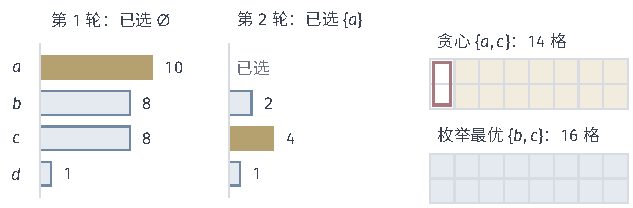
\includegraphics[width=107.177mm]{figures/01-basic-mathematics/04-graphs/tikz/c4-greedy-rounds-vs-optimum/figure.pdf}
  \caption{传感器实例上$k=2$的边际增益贪心。左侧两栏是两轮中各候选元素的当前增益，黄色条为该轮选中的元素；第$2$轮的增益相对于已选的$\{a\}$计算。右侧比较两个覆盖结果：贪心集合$\{a,c\}$（黄色）漏掉第$1$列两格（红框），枚举最优集合$\{b,c\}$（蓝色）覆盖全部$16$格。}
  \label{fig:graph-setfn-greedy-rounds}
\end{figure}

这条轨迹也说明为什么不能只按初始增益排序一次。初始增益的次序是$a$，然后$b,c$并列；按编号取前两个得到$\{a,b\}$，只覆盖$12$格。第$2$轮重新计算后，$b$的增益从$8$降到$2$，$c$的增益从$8$降到$4$，排序已经改变。

\paragraph{求值次数与缓存}
第$t$轮要对$n-t+1$个未选元素各求值一次，总共
\[
  \sum_{t=1}^{k}(n-t+1)\leq nk
\]
次求值，再加上开始时的一次$F(\varnothing)$。传感器实例$n=4$、$k=2$，共$4+3=7$次。若一次求值的代价为$\tau$（例如覆盖量需要合并若干覆盖范围），总代价是$O(nk\tau)$。

对次模函数，可以缓存上一轮算出的增益来减少求值。由式~\eqref{eq:graph-setfn-diminishing-returns}，已选集合变大后，每个元素的增益只会变小，所以旧增益是新增益的上界。每轮把候选元素按缓存值排序，只重新计算排在最前的元素；若它的新增益仍不小于其余元素的缓存值，它就是本轮增益最大者，其余元素不必重算。这种做法的正确性依赖次模性；对一般函数，旧增益不是上界，必须每轮全部重新计算。

\subsection{贪心保证与适用范围}
\label{sec:graph-setfn-greedy-guarantee}

贪心在传感器实例上没有找到最优解，但$14$与$16$相差不多。下面的定理说明这不是巧合：对归一化、单调、次模的目标，贪心值总能达到最优值的一个固定比例。

\begin{theorem}[贪心的近似保证]
\label{thm:graph-setfn-greedy-guarantee}
设$F$是有限底集$V$上的集合函数，满足$F(\varnothing)=0$、单调非减且次模；整数$1\leq k\leq|V|$。记$\mathrm{OPT}$为问题~\eqref{eq:graph-setfn-cardinality-problem}的最优值，$S_\ell$为算法~\ref{alg:graph-setfn-greedy}执行$\ell$轮后的集合（$0\leq\ell\leq k$）。则
\[
  F(S_\ell)\geq\Bigl(1-\bigl(1-\tfrac1k\bigr)^{\ell}\Bigr)\mathrm{OPT}.
\]
特别地，$F(S_k)\geq\bigl(1-(1-1/k)^k\bigr)\mathrm{OPT}\geq(1-e^{-1})\mathrm{OPT}$。
\end{theorem}

\begin{proof}
固定一个最优集合$O$，$|O|\leq k$，$F(O)=\mathrm{OPT}$。考察第$t$轮开始时的集合$S_{t-1}$（$1\leq t\leq k$），先用次模性把它与最优值的差距上界为若干个边际增益之和。把$O\setminus S_{t-1}$中的元素排成$o_1,\ldots,o_r$，由单调性和式~\eqref{eq:graph-setfn-telescoping}，
\[
  \mathrm{OPT}=F(O)\leq F(O\cup S_{t-1})
  =F(S_{t-1})+\sum_{j=1}^{r}\Delta\bigl(o_j\mid S_{t-1}\cup\{o_1,\ldots,o_{j-1}\}\bigr).
\]
每个$o_j$都不在$S_{t-1}\cup\{o_1,\ldots,o_{j-1}\}$中，由式~\eqref{eq:graph-setfn-diminishing-returns}，第$j$项不超过$\Delta(o_j\mid S_{t-1})$。而贪心在第$t$轮选的是增益最大的元素，所以$\Delta(o_j\mid S_{t-1})\leq\Delta(v_t\mid S_{t-1})=F(S_t)-F(S_{t-1})$。又$r\leq|O|\leq k$，且每一项增益非负，于是
\[
  \mathrm{OPT}-F(S_{t-1})\leq k\bigl(F(S_t)-F(S_{t-1})\bigr).
\]
这一步说的是：最优集合至多$k$个元素，它们合起来能补上的差距，至少有$1/k$能被当前最好的单个元素补上。

记差距$\delta_t=\mathrm{OPT}-F(S_t)$。上式可写成$\delta_{t-1}\leq k(\delta_{t-1}-\delta_t)$，即
\[
  \delta_t\leq\Bigl(1-\frac1k\Bigr)\delta_{t-1},\qquad t=1,\ldots,k.
\]
由$F(\varnothing)=0$得$\delta_0=\mathrm{OPT}$，连续使用$\ell$次得$\delta_\ell\leq(1-1/k)^\ell\,\mathrm{OPT}$，移项即为所求。

最后比较$(1-1/k)^k$与$e^{-1}$。函数$\psi(x)=e^{-x}-(1-x)$满足$\psi(0)=0$，导数$\psi'(x)=1-e^{-x}$在$x>0$时为正，所以$\psi$在$[0,+\infty)$上单调递增（第~\ref{sec:ru-monotonicity-convexity}节），从而$0\leq1-x\leq e^{-x}$对$0\leq x\leq1$成立。取$x=1/k$再求$k$次幂，得到$(1-1/k)^k\leq e^{-1}$。
\end{proof}

几个条件各有作用。归一化保证差距从$\mathrm{OPT}$开始；若$F(\varnothing)\neq0$，比例式会因为一个常数而失去意义。单调性用在$F(O)\leq F(O\cup S_{t-1})$和增益非负两处，次模性用在把$O$中元素的增益统一换成相对于$S_{t-1}$的增益。$k=1$时界为$1$，贪心选出的就是最好的单元素；$k=2$时界为$3/4$，传感器实例中$14\geq\frac34\times16=12$，与定理一致。$1-e^{-1}\approx0.632$是对一切$k$都成立的下界。

\paragraph{撤去次模性}
图~\ref{fig:graph-setfn-property-counterexamples}(a)的函数$F(S)=\max\{3\,\mathbb I\{\{1,2\}\subseteq S\},\mathbb I\{3\in S\}\}$单调、归一化，但不是次模的。取$k=2$：第$1$轮三个增益依次为$0,0,1$，选$3$；第$2$轮相对于$\{3\}$，加入$1$或$2$的增益都是$0$，按编号选$1$，得到$F(\{1,3\})=1$。最优集合是$\{1,2\}$，$\mathrm{OPT}=3$。元素$1,2$只有同时选中才有价值，每一轮单独看它们的增益都是零，贪心永远看不到这个互补组合。把$3$换成任意大的$M$，比例$1/M$可以任意小，所以没有次模性就没有固定比例的保证。

\paragraph{撤去单调性}
图~\ref{fig:graph-setfn-property-counterexamples}(b)的单边割权是次模的，但不单调。取$k=2$并按算法~\ref{alg:graph-setfn-greedy}强制选满：第$1$轮选$1$（增益$1$），第$2$轮只剩$2$，增益为$-1$，仍须加入，结果$\operatorname{cut}(\{1,2\})=0$，而至多选两个时的最优值是$1$。在增益为负时停止可以避免这个例子中的损失，但对一般的非单调次模函数，这样修改后的贪心仍没有定理~\ref{thm:graph-setfn-greedy-guarantee}那样的保证，需要另外的算法与分析，本节不展开。

因此，定理~\ref{thm:graph-setfn-greedy-guarantee}只适用于本节规定的问题：在基数约束下最大化归一化、单调、次模的集合函数。它给出的是近似比例，不是精确最优性；目标、约束或函数性质改变时，都需要重新论证。
